\section{Neural Networks}

\begin{enumerate}[label=2.\arabic*, itemsep=8pt]
	\item Logische poorten
	\begin{enumerate}[itemsep=8pt]
		\item De inputs/output geven de waarheidstabel van een AND-poort:
		\begin{itemize}
			\item $x_1 = 0$; $x_2 = 0$ geeft $0 \times 0.5 + 0 \times 0.5 - 1.0 = -1.0 < 0$ dus $g = 0$
			\item $x_1 = 0$; $x_2 = 1$ geeft $0 \times 0.5 + 1 \times 0.5 - 1.0 = -0.5 < 0$ dus $g = 0$
			\item $x_1 = 1$; $x_2 = 0$ geeft $1 \times 0.5 + 0 \times 0.5 - 1.0 = -0.5 < 0$ dus $g = 0$
			\item $x_1 = 1$; $x_2 = 1$ geeft $1 \times 0.5 + 1 \times 0.5 - 1.0 = 0.0 = 0$ dus $g = 1$
		\end{itemize}

		\item De inputs/output geven de waarheidstabel van een OR-poort:
		\begin{itemize}
			\item $x_1 = 0$; $x_2 = 0$ geeft $0 \times 0.5 + 0 \times 0.5 - 0.5 = -0.5 < 0$ dus $g = 0$
			\item $x_1 = 0$; $x_2 = 1$ geeft $0 \times 0.5 + 1 \times 0.5 - 0.5 = 0.0 = 0$ dus $g = 1$
			\item $x_1 = 1$; $x_2 = 0$ geeft $1 \times 0.5 + 0 \times 0.5 - 0.5 = 0.0 = 0$ dus $g = 1$
			\item $x_1 = 1$; $x_2 = 1$ geeft $1 \times 0.5 + 1 \times 0.5 - 0.5 = 0.5 > 0$ dus $g = 1$
		\end{itemize}

		\item De input/output geeft de waarheidstabel van een INVERT-poort (met andere woorden, de logische NOT):
		\begin{itemize}
			\item $x_1 = 0$ geeft $0 \times -1 + 0.5 = 0.5 > 0$ dus $g = 1$
			\item $x_1 = 1$ geeft $1 \times -1 + 0.5 = -0.5 < 0$ dus $g = 0$
		\end{itemize}	
	\end{enumerate}


	\item PARTY-poort
	\begin{enumerate}[itemsep=8pt]
		\item Bijvoorbeeld: $x_1 = x_2 = x_3 = 1$ geeft \\ $1 \times 0.6 + 1 \times 0.3 + 1 \times 0.2 - 0.4 = 0.7 > 0$ dus $g = 1$

		\begin{tabular}{c|c|c|c|c}
		      $x_1$ 			& $x_2$ 			& $x_3$			& gewogen som			& $g$	\\
		      \hline
		      0				& 0				& 0 				& $-0.4 < 0$			& 0		\\
		      0				& 0				& 1 				& $-0.2 < 0$			& 0		\\
		      0				& 1				& 0 				& $-0.1 < 0$			& 0		\\
		      0				& 1				& 1 				& $0.1 > 0$			& 1		\\
		      1				& 0				& 0 				& $0.2 > 0$			& 1		\\
		      1				& 0				& 1 				& $0.4 > 0$			& 1		\\
		      1				& 1				& 0 				& $0.5 > 0$			& 1		\\
		      1				& 1				& 1 				& $0.7 > 0$			& 1		\\
	    \end{tabular}

	    	\item Bijvoorbeeld: $x_1 = x_2 = x_3 = 1$ geeft \\ $1 \times 0.1 + 1 \times 0.3 + 1 \times 0.2 - 0.9 = -0.3 < 0$ dus $g = 0$

		\begin{tabular}{c|c|c|c|c}
		      $x_1$ 			& $x_2$ 			& $x_3$			& gewogen som			& $g$	\\
		      \hline
		      0				& 0				& 0 				& $-0.9 < 0$			& 0		\\
		      0				& 0				& 1 				& $-0.7 < 0$			& 0		\\
		      0				& 1				& 0 				& $-0.6 < 0$			& 0		\\
		      0				& 1				& 1 				& $-0.4 < 0$			& 0		\\
		      1				& 0				& 0 				& $-0.8 < 0$			& 0		\\
		      1				& 0				& 1 				& $-0.6 < 0$			& 0		\\
		      1				& 1				& 0 				& $-0.5 < 0$			& 0		\\
		      1				& 1				& 1 				& $-0.3 < 0$			& 0		\\
	    \end{tabular}
    	\end{enumerate}


	\item NOR-poort: zie figuur \ref{fig:nor_gate}.
		\begin{figure}[h!]
		\centering
		\begin{tikzpicture}[scale=1, transform shape]
			\node (a)[circle, draw] at (4, 0) {$b = 0.0$};
			\node (x1)[] at (0, 2) {$x_1$};
			\node (x2)[] at (0, 0) {$x_2$};
			\node (x3)[] at (0, -2) {$x_3$};
			\node (output)[] at (7, 0) {output};
			\draw[->] (x1) -- (a) node[pos=0.3,sloped,above] {\small $w_1 = -1$};
			\draw[->] (x2) -- (a) node[pos=0.35,sloped,above] {\small $w_2 = -1$};
			\draw[->] (x3) -- (a) node[pos=0.4,sloped,above] {\small $w_3 = -1$};
			\draw[->] (a) -- (output);
		\end{tikzpicture}
		\caption{Oplossing NOR-poort}
		\label{fig:nor_gate}
		\end{figure}



	\item XOR-poort: zie figuur \ref{fig:xor_gate}.
		\begin{figure}
		\centering
		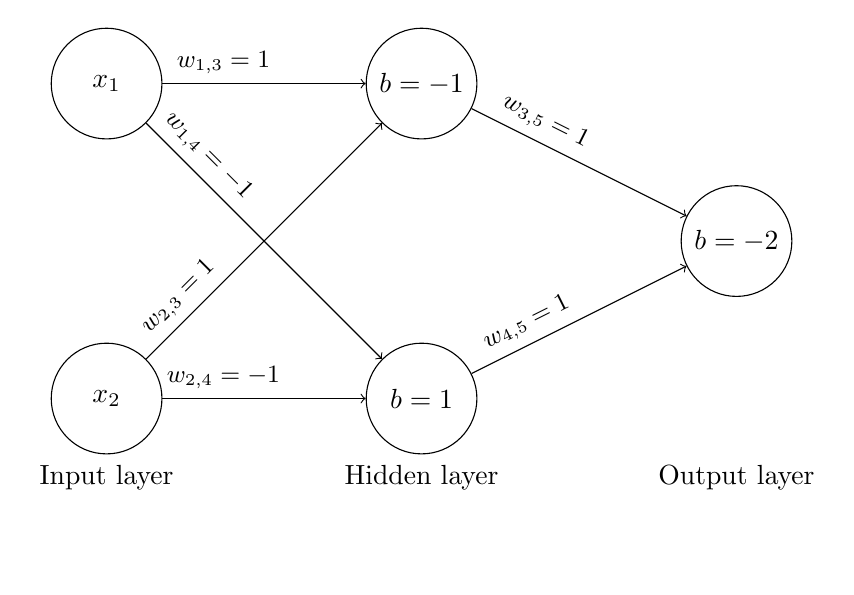
\begin{tikzpicture}[scale=1, transform shape]
			\node (x1)[circle, draw, minimum width=40pt] at (0, 2) {$x_1$};
			\node (x2)[circle, draw, minimum width=40pt] at (0, -2) {$x_2$};
			\node (IL)[circle] at (0, -3) {Input layer};

			\node (a)[circle, draw, minimum width=40pt] at (4, 2) {$b = -1$};
			\node (b)[circle, draw, minimum width=40pt] at (4, -2) {$b = 1$};
			\node (HL)[circle] at (4, -3) {Hidden layer};

			\node (c)[circle, draw, minimum width=40pt] at (8, 0) {$b = -2$};
			\node (OL)[circle] at (8, -3) {Output layer};

			\draw[->] (x1) -- (a) node[pos=0.3,sloped,above] {\small $w_{1,3} =  1$};
			\draw[->] (x1) -- (b) node[pos=0.2,sloped,above] {\small $w_{1,4} = -1$};
			\draw[->] (x2) -- (a) node[pos=0.2,sloped,above] {\small $w_{2,3} =  1$};
			\draw[->] (x2) -- (b) node[pos=0.3,sloped,above] {\small $w_{2,4} = -1$};

			\draw[->] (a) -- (c) node[pos=0.3,sloped,above] {\small $w_{3,5} = 1$};
			\draw[->] (b) -- (c) node[pos=0.3,sloped,above] {\small $w_{4,5} = 1$};
		\end{tikzpicture}
		\caption{Oplossing XOR-poort: de bovenste node van de hidden layer is een OR-poort en de onderste is een NAND-poort; de outputnode is een AND-poort.}
		\label{fig:xor_gate}
		\end{figure}


	\item Half adder: zie figuur \ref{fig:adder}.
		\begin{figure}
		\centering
		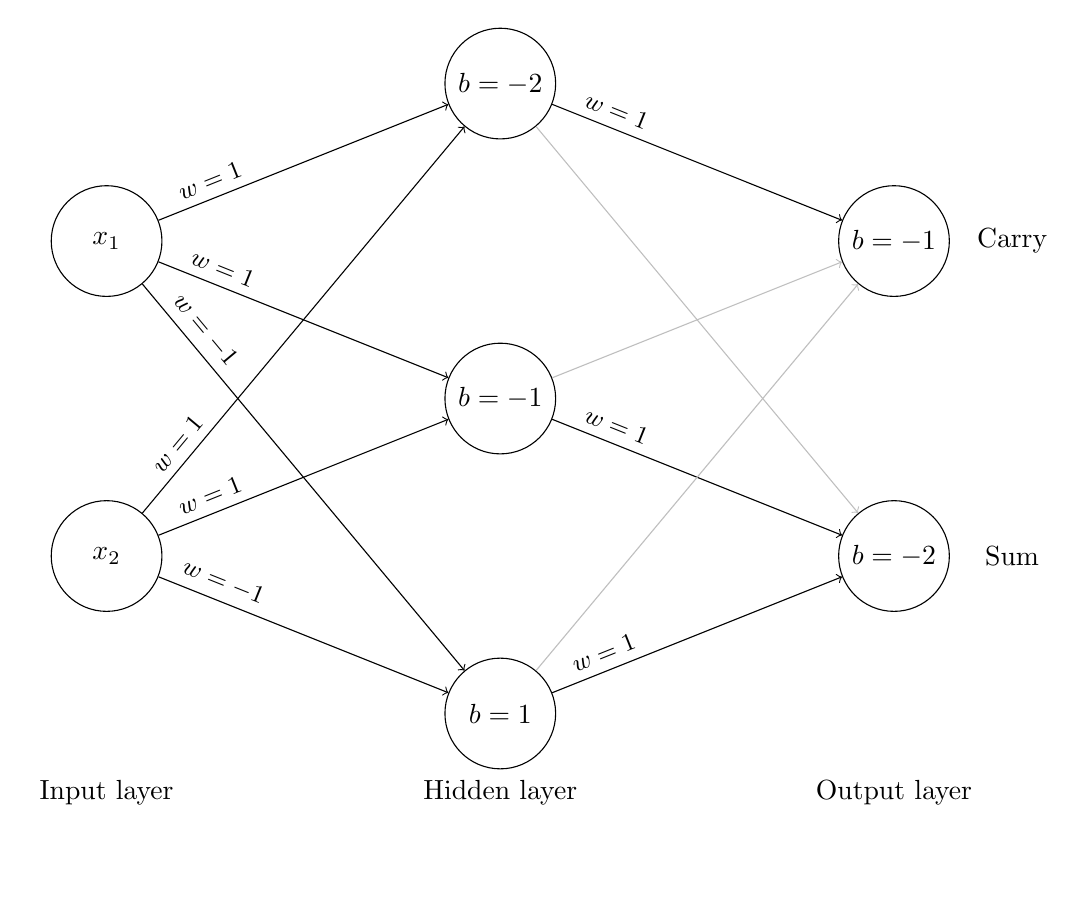
\begin{tikzpicture}[scale=1, transform shape]
			\node (x1)[circle, draw, minimum width=40pt] at (0, 2) {$x_1$};
			\node (x2)[circle, draw, minimum width=40pt] at (0, -2) {$x_2$};
			\node (IL)[circle] at (0, -5) {Input layer};

			\node (f)[circle, draw, minimum width=40pt] at (5, 4) {$b = -2$};
			\node (g)[circle, draw, minimum width=40pt] at (5, 0) {$b = -1$};
			\node (h)[circle, draw, minimum width=40pt] at (5, -4) {$b = 1$};
			\node (HL)[circle] at (5, -5) {Hidden layer};

			\node (c)[circle, draw, minimum width=40pt] at (10, 2) {$b = -1$};
			\node (CL)[circle] at (11.5, 2) {Carry};
			\node (s)[circle, draw, minimum width=40pt] at (10, -2) {$b = -2$};
			\node (SL)[circle] at (11.5, -2) {Sum};
			\node (OL)[circle] at (10, -5) {Output layer};


			\draw[->] (x1) -- (f) node[pos=0.2,sloped,above] {\small $w = 1$};
			\draw[->] (x1) -- (g) node[pos=0.2,sloped,above] {\small $w = 1$};
			\draw[->] (x1) -- (h) node[pos=0.15,sloped,above] {\small $w = -1$};
			\draw[->] (x2) -- (f) node[pos=0.15,sloped,above] {\small $w = 1$};
			\draw[->] (x2) -- (g) node[pos=0.2,sloped,above] {\small $w = 1$};
			\draw[->] (x2) -- (h) node[pos=0.2,sloped,above] {\small $w = -1$};

			\draw[->] (f) -- (c) node[pos=0.2,sloped,above] {\small $w =  1$};
			\draw[->, lightgray] (f) -- (s) node[pos=0.2,sloped,above] {};
			\draw[->, lightgray] (g) -- (c) node[pos=0.2,sloped,above] {};
			\draw[->] (g) -- (s) node[pos=0.2,sloped,above] {\small $w =  1$};
			\draw[->, lightgray] (h) -- (c) node[pos=0.2,sloped,above] {};
			\draw[->] (h) -- (s) node[pos=0.2,sloped,above] {\small $w = 1$};
		\end{tikzpicture}
		\caption{Oplossing half-adder. De sum is een XOR en de carry is een AND. De bovenste outputnode is de carry en de onderste is de sum. De bovenste hidden node is de AND en de carry zelf doet niets. De onderste twee hidden nodes en de sumnode zijn samen een XOR (zie boven). De grijze verbindingen hebben $w=0$.}
		\label{fig:adder}
		\end{figure}


	\item Bitwise representation: zie figuur \ref{fig:bitwise}.
		\begin{figure}
		\centering
		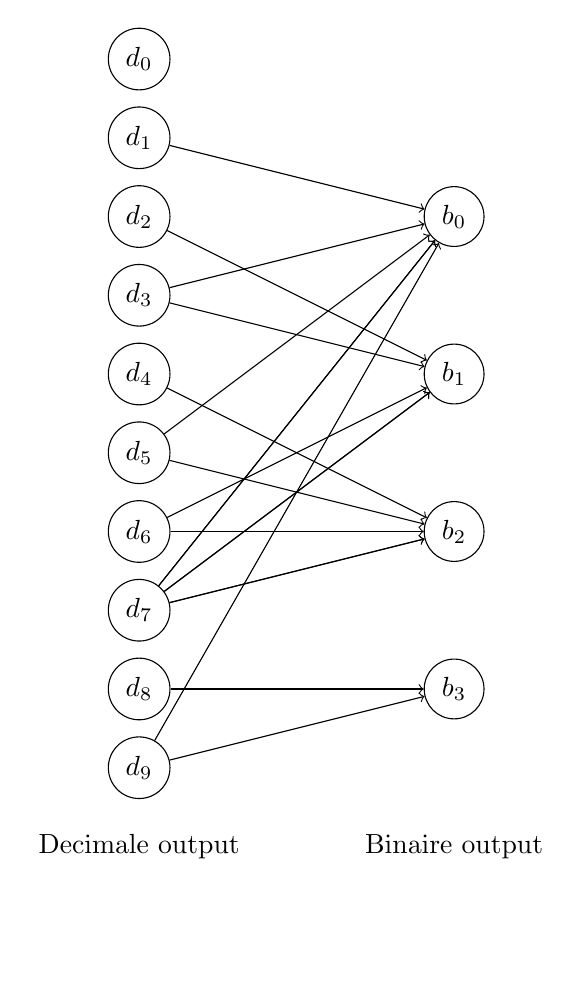
\begin{tikzpicture}[scale=1, transform shape]
			\node (x0)[circle, draw] at (0,  0) {$d_0$};
			\node (x1)[circle, draw] at (0, -1) {$d_1$};
			\node (x2)[circle, draw] at (0, -2) {$d_2$};
			\node (x3)[circle, draw] at (0, -3) {$d_3$};
			\node (x4)[circle, draw] at (0, -4) {$d_4$};
			\node (x5)[circle, draw] at (0, -5) {$d_5$};
			\node (x6)[circle, draw] at (0, -6) {$d_6$};
			\node (x7)[circle, draw] at (0, -7) {$d_7$};
			\node (x8)[circle, draw] at (0, -8) {$d_8$};
			\node (x9)[circle, draw] at (0, -9) {$d_9$};
			\node (IL)[circle] at (0, -10) {Decimale output};

			\node (b1)[circle, draw] at (4, -2) {$b_0$};
			\node (b2)[circle, draw] at (4, -4) {$b_1$};
			\node (b3)[circle, draw] at (4, -6) {$b_2$};
			\node (b4)[circle, draw] at (4, -8) {$b_3$};
			\node (HL)[circle] at (4, -10) {Binaire output};

			\draw[->] (x1) -- (b1) node[pos=0.2,sloped,above] {};
			\draw[->] (x2) -- (b2) node[pos=0.2,sloped,above] {};
			\draw[->] (x3) -- (b1) node[pos=0.15,sloped,above] {};
			\draw[->] (x3) -- (b2) node[pos=0.15,sloped,above] {};
			\draw[->] (x4) -- (b3) node[pos=0.15,sloped,above] {};
			\draw[->] (x5) -- (b1) node[pos=0.15,sloped,above] {};
			\draw[->] (x5) -- (b3) node[pos=0.15,sloped,above] {};
			\draw[->] (x6) -- (b2) node[pos=0.15,sloped,above] {};
			\draw[->] (x6) -- (b3) node[pos=0.15,sloped,above] {};
			\draw[->] (x7) -- (b1) node[pos=0.15,sloped,above] {};
			\draw[->] (x7) -- (b2) node[pos=0.15,sloped,above] {};
			\draw[->] (x7) -- (b3) node[pos=0.15,sloped,above] {};
			\draw[->] (x7) -- (b1) node[pos=0.15,sloped,above] {};
			\draw[->] (x7) -- (b2) node[pos=0.15,sloped,above] {};
			\draw[->] (x7) -- (b3) node[pos=0.15,sloped,above] {};
			\draw[->] (x8) -- (b4) node[pos=0.15,sloped,above] {};
			\draw[->] (x9) -- (b1) node[pos=0.15,sloped,above] {};
			\draw[->] (x9) -- (b4) node[pos=0.15,sloped,above] {};
		\end{tikzpicture}
		\caption{Oplossing binary representation. Bias $b = -1$ voor elke $b_i$. De getekende verbindingen hebben allen $w=1$, de ontbrekende verbindingen hebben allen $w=0$.}
		\label{fig:bitwise}
		\end{figure}

\end{enumerate}

% Opgave 4.2
% De sigmoid geeft de volgende resultaten:
 % x1  x2   AND (2.5)  OR (2.6)
 % 0   0   0.26894    0.37754
 % 0   1   0.37754    0.50000
 % 1   0   0.37754    0.50000
 % 1   1   0.50000    0.62246

% Het probleem is dat wanneer de som gelijk is aan 0, de sigmoid op 0.5 blijft hangen. Je moet dus meer op zoek naar de extremen:
% - Voor de AND komt een netwerk w = [2, 2] met b = -3 al beter in de buurt.
% - Voor de OR komt een netwerk w = [2, 2] met b = -1 al beter in de buurt.

% Vermenigvuldig bovenstaande parameters met een grote factor en je krijgt een output met 0'en en 1'en.
